\documentclass[12pt]{article}
\usepackage{graphicx}


\title{Assignment 4}
\date{}
\author{}
\begin{document}
\maketitle

\section{AE22B008:- }
\begin{itemize}
    \item \textbf{Name:- } \underline{\textit{U.Shriram}}
    \item \textbf{Github user id:}- 132140196
\end{itemize}
    The equation i am going to write about is the equation of Normal Distribution.This distribution is also known as the Gaussian distribution, named after C.F Gauss.The normal distribution is the most important probability distribution in statistics.The equation is as follows:- 
\bigskip    
\begin{equation}
    \Large f(x,\mu,\sigma^2)=\frac{1}{\sigma\sqrt{2\pi}}e^{(\frac{-1}{2}(\frac{x-\mu}{\sigma})^2)} 
\end{equation}
\begin{itemize}
    \item x = value of the variable or data being examined and f(x) the probability function
    \item $\mu$ = the mean
    \item $\sigma$ = the standard deviation
\end{itemize}

\bigskip
Gaussian distribution is symmetric about the mean showing that data near the mean are more frequent in occurrence than data far from the mean.

\medskip
The normal distribution depends on two parameters: the mean $\mu$ and the standard deviation $\sigma$. These two parameters define the shape and probabilities of the normal distribution entirely. 

\medskip
The mean defines the location of the peak for the normal distribution, and the standard deviation defines the width. Extreme values in both tails of the distribution are similarly unlikely.

\begin{figure}[ht]
    \centering
    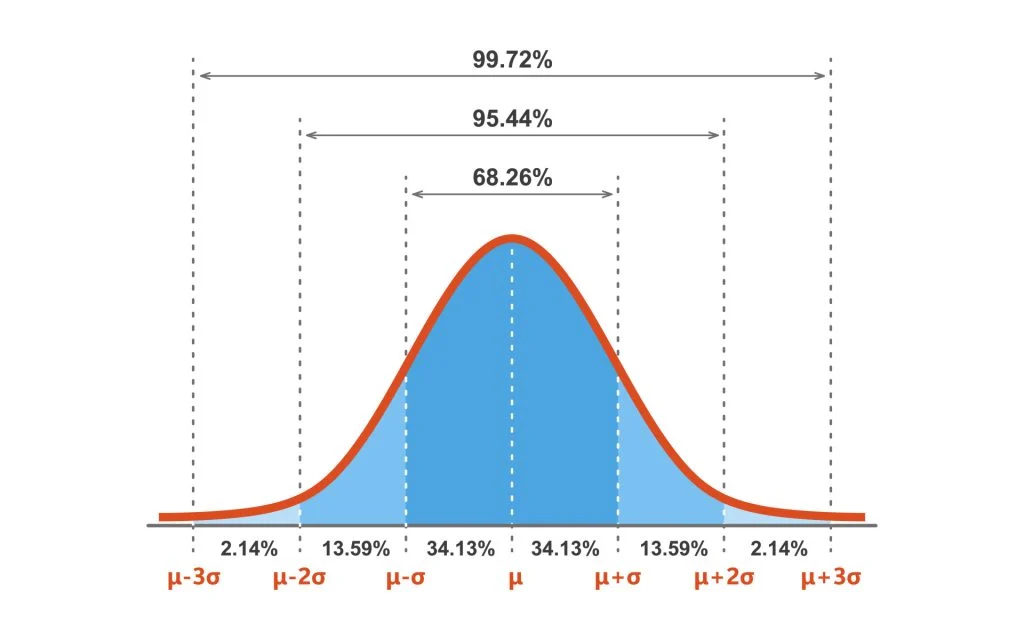
\includegraphics[width=1\textwidth]{bell_curve.jpg}
    \caption{Normal distribution.}
    \label{fig:mesh1}
\end{figure}


Many naturally-occurring phenomena appear to be normally-distributed. Take, for example, the distribution of the heights of human beings, IQ scores measurement etc.There are a number of applications of normal curve in the field of measurement and evaluation in psychology and education.

\medskip
While learning about logistic and linear regression i found out that linear regression and logistic regression models often assume that the errors or residuals follow a Gaussian distribution.Assuming the errors to be a Gaussian function allows for the use of maximum likelihood estimation (MLE) to estimate the model parameters, such as the coefficients.It ensures that the estimated coefficients are unbiased and have the minimum variance.

\medskip
Other forms of the Gaussian formulae includes one in Brownian motion where the probability density function (PDF) of the displacement at a given time follows a Gaussian distribution

\bigskip    
\begin{equation}
    \Large P(x,t)=\frac{1}{\sqrt{4\pi Dt}}e^{-(\frac{x^2}{4Dt})}
\end{equation}
\begin{itemize}
    \item x = displacement of particle
    \item D = Diffusion coefficient 
    \item t = time
\end{itemize}

\bigskip
According to \cite{Uhlenbeck1930}, the theory of Brownian motion was discussed.\footnote{\bibliography{bi}
\bibliographystyle{alpha}}

\medskip
According to \cite{terBraak1986}, the topics of Weighted averaging, logistic regression and the Gaussian response model were discussed.\footnote{}
\end{document}
